\documentclass[conference]{IEEEtran}
\IEEEoverridecommandlockouts
% The preceding line is only needed to identify funding in the first footnote. If that is unneeded, please comment it out.
\usepackage{cite}
\usepackage{amsmath,amssymb,amsfonts}
\usepackage{algorithmic}
\usepackage{graphicx}
\usepackage{textcomp}
\usepackage{xcolor}
\usepackage{hyperref}
\usepackage{subfig}
%\DeclareUnicodeCharacter{200B}{I~AM~HERE!!!!}

\def\BibTeX{{\rm B\kern-.05em{\sc i\kern-.025em b}\kern-.08em
    T\kern-.1667em\lower.7ex\hbox{E}\kern-.125emX}}
\begin{document}

\title{Sistemi e Architetture per Big Data - AA 2020/2021 \\
	\LARGE \emph{Secondo progetto}}

\author{\IEEEauthorblockN{Giuseppe Lasco}
\IEEEauthorblockA{\textit{Dipartimento di Ingegneria dell'Informazione} \\
\textit{Universit\`{a} degli studi di Roma "Tor Vergata"
}\\
Roma, Italia \\
giuseppe.lasco17@gmail.com}
\and
\IEEEauthorblockN{Marco Marcucci}
\IEEEauthorblockA{\textit{Dipartimento di Ingegneria dell'Informazione} \\
\textit{Universit\`{a} degli studi di Roma "Tor Vergata"
}\\
Roma, Italia \\
marco.marcucci96@gmail.com}

}

\maketitle

\begin{abstract}
Questo documento riporta i dettagli implementativi
riguardanti l'analisi mediante \emph{Flink} del dataset relativo a dati provenienti da
dispositivi Automatic Identification System (AIS) contenenti informazioni riguardo lo stato di navi in movimento per garantire la sicurezza di quest'ultime in mare e nei porti. Viene, inoltre, descritta l'architettura
a supporto dell'analisi e gli ulteriori \emph{framework} utilizzati.
\end{abstract}

\section{\textbf{Introduzione}}
L'analisi effettuata si pone lo scopo di rispondere a delle
query relative a classifiche e statistiche riguardanti le navi e le tratte presenti nel dataset.\\

\subsection*{\textbf{Dataset}} 
Il dataset preso in considerazione \`{e} \textit{prj2\_dataset.csv}, il quale contiene dati rigurdanti gli identificativi e le caratteristiche istantanee delle navi e delle tratte. I campi di interesse sono:
\begin{itemize}
\item \textbf{ID}: stringa esadecimale che rappresenta l’identificativo della nave;
\item \textbf{SHIP TYPE}: numero intero che rappresenta la tipologia della nave
\item \textbf{LON}: numero in virgola mobile che rappresenta la coordinata cartesiana in gradi decimali della
longitudine data dal GPS;
\item \textbf{LAT}: numero in virgola mobile che rappresenta la coordinata cartesiana in gradi decimali della latitudine data dal sistema GPS;
\item \textbf{TIMESTAMP}: rappresenta l’istante temporale della segnalazione dell’evento AIS; il timestamp è
espresso con il formato GG-MM-YY hh:mm:ss (giorno, mese, anno, ore, minuti e secondi dell’evento);
\item \textbf{TRIP ID}: stringa alfanumerica che rappresenta l’identificativo del viaggio; è composta dai primi 7
caratteri (inclusi 0x) di SHIP ID, concatenati con la data di partenza e di arrivo.
\end{itemize}
\par La
frequenza di produzione di tali dati è in funzione dello stato di moto, con un periodo temporale variabile tra i 2 secondi in fase di manovra a 5 minuti in fase di navigazione ad alta velocità. Inoltre, l'area marittima è limitata alla zona del Mar Mediterraneo descritta dalle seguente coordinate: LON $\in$ [-6.0, 37.0] LAT $\in$ [32.0, 45.0].
Tale area è stata suddivisa in celle rettangolari di uguale dimensione; i settori di LAT vengono identificati dalle lettere che vanno da A a J, mentre i settori di LON dai numeri interi che vanno da 1 a 40. Ad ogni cella è associato un \emph{id} dato dalla combinazione della lettera del
settore LAT e dal numero di settore LON.
\subsection*{\textbf{Query}}
L'obiettivo di questo progetto \`{e} quello di implementare ed eseguire tre query utilizzando \emph{Flink}.

\par La prima query ha come scopo quello di calcolare, per il Mar Mediterraneo Occidentale, il numero medio giornaliero  di navi militari, navi per trasporto passeggeri, navi cargo e le restanti tipologie, utilizzando finestre temporali di tipo \emph{Tumbling} da 7 giorni e da 1 mese.

\par La seconda query consiste nel determinare le prime 3 celle per le quali il grado di frequentazione \`{e} pi\`{u} alto, nelle due fascie orarie 00:00-11:59 e 12:00-23:59, Mar Mediterraneo Occidentale ed Orientale. il grado di frequentazione di una cella viene calcolato come il numero di navi diverse che attraversano la cella nella fascia oraria in esame. Sono state utilizzate finestre temporali a 7 giorni e 1 mese.

\par L'ultima query consiste nel determinare le prime 5 tratte per cui la distanza percorsa fino a quel momento \`{e} pi\`{u} alta. Per il calcolo della distanza è stata considerata la distanza euclidea.

\subsection*{\textbf{Framework}}
Come \emph{framework} di processamento stream \`{e} stato utilizzato \emph{Apache Flink} che riceve i dati dal sistema di messaging \emph{Apache Kafka}. 

\section{\textbf{Architettura}}
L'architettura si compone di due container \emph{Docker}, su cui eseguono i servizi di \emph{Apache Zookeeper} e \emph{Apache Kafka} che comunicano tra di loro attraverso la stessa rete, creata appositamente dal servizio \emph{Docker Compose}. Inoltre, sempre sulla stessa macchina, una JVM ospita l'esecuzione di \emph{Apache Flink} e un processo \emph{Java} immette i dati nel sistema di Publish/Subscribe.

\begin{figure}[htbp]
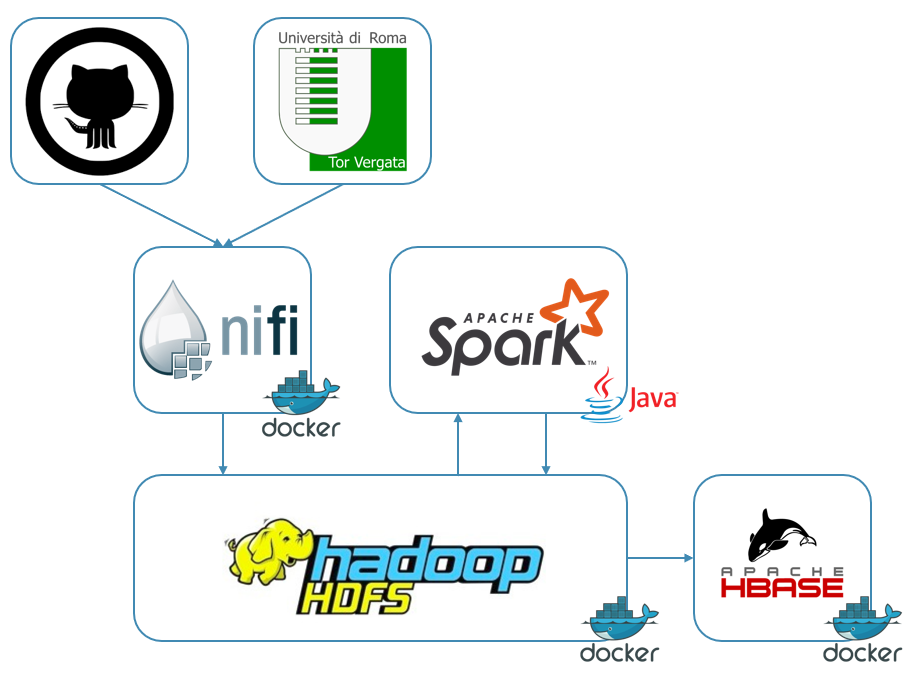
\includegraphics[scale=0.36]{Screenshot/arch.png}
\caption{Schema dell'architettura}\label{figura:architettura}
\label{fig}
\end{figure}

\subsection*{\textbf{Producer}}
Il Producer si occupa di leggere il ​dataset, mantenuto in un
file CSV locale, e di pubblicarne il contenuto presso il
topiche di Kafka (query) da cui \emph{Flink} recupera i dati. La scrittura sulla
topica viene effettuata riga per riga a intervalli variabili, proporzionali ai timestamp reali presenti nel dataset, al fine di simulare una
vera sorgente di dati ​real time ​accelerata. L'ordinamento del dataset \`{e} stato effettuato utilizzando una struttura dati che permette di ordinare all'inserimento dei record, ovvero la \emph{TreeMap}. La gestione di chiavi uguali (timestamp) \`{e} stata effettuata utilizzando come valore della coppia key-value della \emph{TreeMap}, una lista, popolata dai record da inviare, in modo da non perdere occorrenze.
Per garantire la corretta esecuzione del processamento su
\emph{Flink} in base all'​ event time,​ \`{e} stato necessario
estrarre la data di occorrenza dell'evento di ogni riga e
impostarla come ​timestamp della relativa tupla alla
pubblicazione sulla topica. 

\subsection*{\textbf{Apache Kafka}}
Kafka è il sistema di messaggistica di tipo ​publish-subscribe
utilizzato per l'ingestion di dati nei sistemi di processamento
e per l'export dei risultati. Il ​cluster, realizzato con Docker
Compose, prevede un​ container con Zookeeper, necessario
per la coordinazione, e altri tre​ container con la funzione di
Kafka broker. Sono state create 16 topiche: una per le tuple
in input a Flink, una per le tuple in input a Kafka Streams,
sei per l'output della prima query (giornaliero, settimanale e
mensile, rispettivamente per Flink e Kafka Streams), quattro
per l'output della seconda ​query (giornaliero e settimanale,
rispettivamente per Flink e Kafka Streams) e altrettante per
quello della terza query. Per incrementare la tolleranza ai
guasti, ogni Kafka ​topic è impostata per avere un grado di
replicazione pari a 2 (una replica ​leader ed una replica
follower) e, allo stesso tempo, una sola partizione. La scelta
della singola partizione è dovuta alla necessità di
mantenere le tuple ordinate all’interno del sistema di
messaggistica; in Kafka, infatti, la garanzie di ordinamento
sono valide soltanto nell’ambito di una singola partizione.
\begin{figure}[htbp]
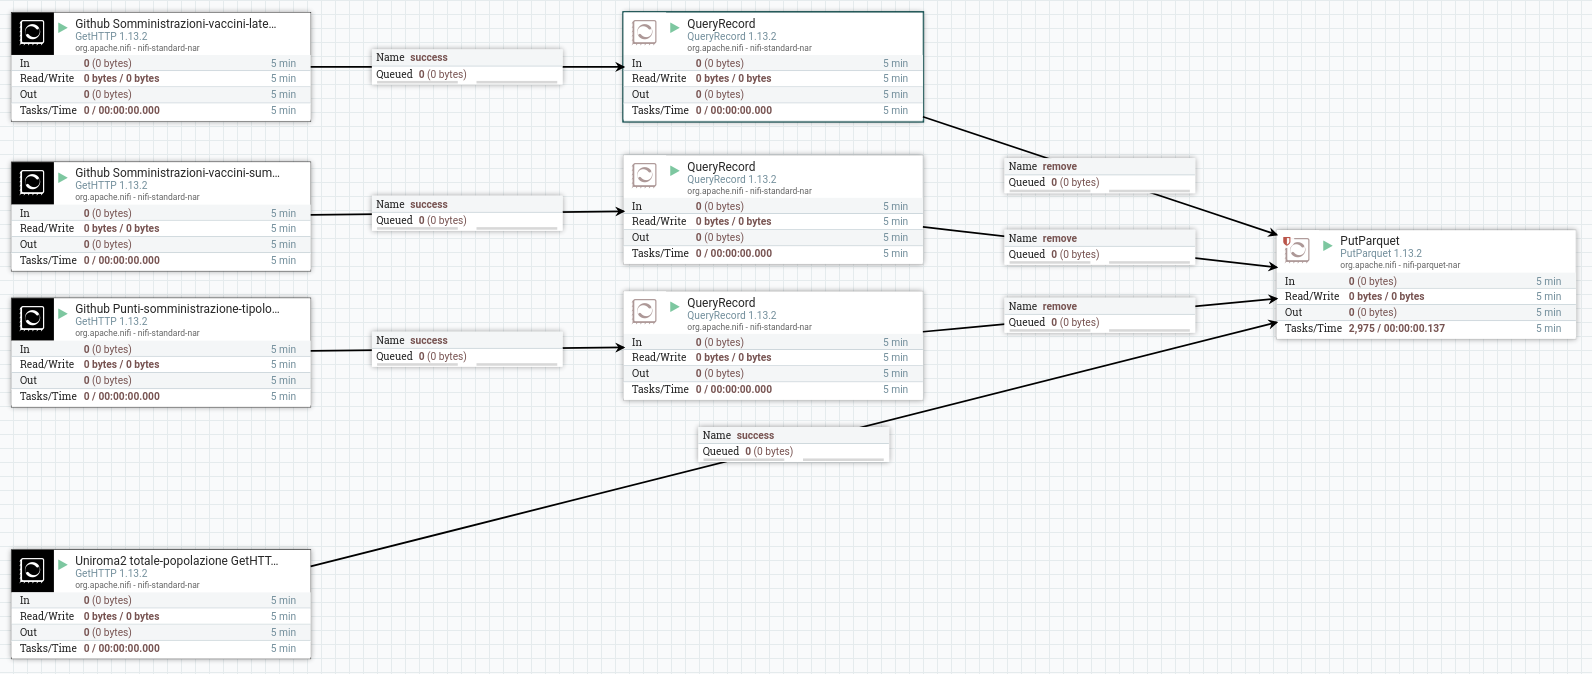
\includegraphics[scale=0.16]{Screenshot/Nifi.png}
\caption{NiFi template}\label{figura:template}
\label{fig}
\end{figure}

\subsection*{\textbf{HDFS}}
\emph{HDFS} rappresenta il mezzo che permette l'archiviazione dei dati in maniera distribuita. Il servizio si compone di un nodo \emph{master} e tre nodi \emph{worker} con un livello di replicazione pari a 2. Tale servizio permette di rendere disponibili i dati su cui \emph{Spark} esegue la computazione e memorizza gli \emph{output} dell'analisi, che vengono, in seguito, esportati su \emph{HBase}, per eventuali analisi, manipolazione e rappresentazione dei dati. Il deployment del framework avviene attraverso l'utilizzo dell'immagine \emph{Docker} \emph{effeerre/hadoop}, istanziata su container. In seguito all'avvio del servizio, uno script permette di eseguire lo sturtup del \emph{Namenode} e dei \emph{Datanode}, e crea le directory \texttt{/data}, dove \emph{NiFi} inserisce i dati, e \texttt{/output}, in cui risiedono i risultati dell'analisi, concedendo i permessi di lettura, scrittura ed esecuzione.

\subsection*{\textbf{Spark}}
Al fine di preprocessare i dati ed eseguire le \emph{query}, viene utilizzato \emph{Apache Spark} in locale, tramite lo script \texttt{\$SPARK\_HOME/bin/spark-submit}. Oltre allo \emph{Spark Core}, che espone un set di API di \emph{trasformazioni} ed \emph{azioni}, \`{e} stata impiegata la libreria di \emph{Machine Learning} \emph{MLlib}, utile per effettuare \emph{clustering} sui risultati della terza \emph{query}.

\subsection*{\textbf{HBase}}
Hbase \`{e} stato utilizzato come datastore \emph{NoSQL} sul quale importare i risultati delle query, anche questo servizio \`{e} stato istanziato utilizzando un container \emph{Docker} realizzato,
questa volta, a partire dall'immagine \emph{harisekhon/hbase}. Affinch\`{e} fosse possibile
l'esportazione dei risultati da \emph{HDFS} a \emph{HBase}, \`{e} stata creata la classe \texttt{HBaseQueries.java} che permette la creazione delle tabelle e l'inserimento dei dati, sfruttando la classe \texttt{HBaseClient.java}. Quest'ultima contiene informazioni riguardo la configurazione di \emph{HBase} e \emph{Zookeeper}, e le principali operazioni di gestione del datastore.\\
\section{\textbf{Query}}
\subsection*{\textbf{Query 1}}
Al fine di soddisfare la seguente \emph{query}, si \`{e} reso necessario l'utilizzo di due file, \textit{somministrazioni-vaccini-summary-latest.parquet} e \textit{punti-somministrazione-tipologia.parquet}. \par
Tali file sono stati caricati in \texttt{Dataset} e trasformati in \texttt{JavaPairRDD}, considerando le sole colonne di interesse: \emph{data\_somministrazione}, \emph{area} e \emph{totale} per il primo e \emph{area} per il secondo. \`{E} stato effettuata la \emph{trasformazione} \emph{"filter"}, scartando i dati precedenti al 1 Gennaio 2021 e successivi al 31 Maggio 2021, seguito da un'ordinamento dell'\texttt{RDD} \textit{somministrazioni-vaccini-summary-latest} in base alla data. Una \emph{trasformazione} di \emph{"reduceByKey"} ha permesso di ottenere il totale di vaccinazioni per ogni mese. Utilizzando un approccio simile al \emph{word count}, sono stati contati i centri riferiti ad una determinata Regione relativi all'\texttt{RDD} \textit{punti-somministrazione-tipologia}. Successivamente, la \emph{"join"} ha permesso di unire i due \texttt{RDD}, utilizzando come chiave la Regione. Il risultato finale \`{e} stato ottenuto dividendo il totale per il numero di giorni del mese di riferimento e per il numero di centri della regione di riferimento, ordinando, infine, il risultato in termini di mese e regione.
\par In figura~\ref{Query1_DAG} \`{e} possibile osservare lo scheduling di Spark dei passi appena descritti attraverso il \emph{DAG}.\par In figura~\ref{Query1_TL} \`{e} possibile osservare \emph{l'event timeline} che descrive il susseguirsi degli eventi rispetto al tempo, evidenziando il parallelismo di alcune operazioni. 
\begin{figure}[htbp]
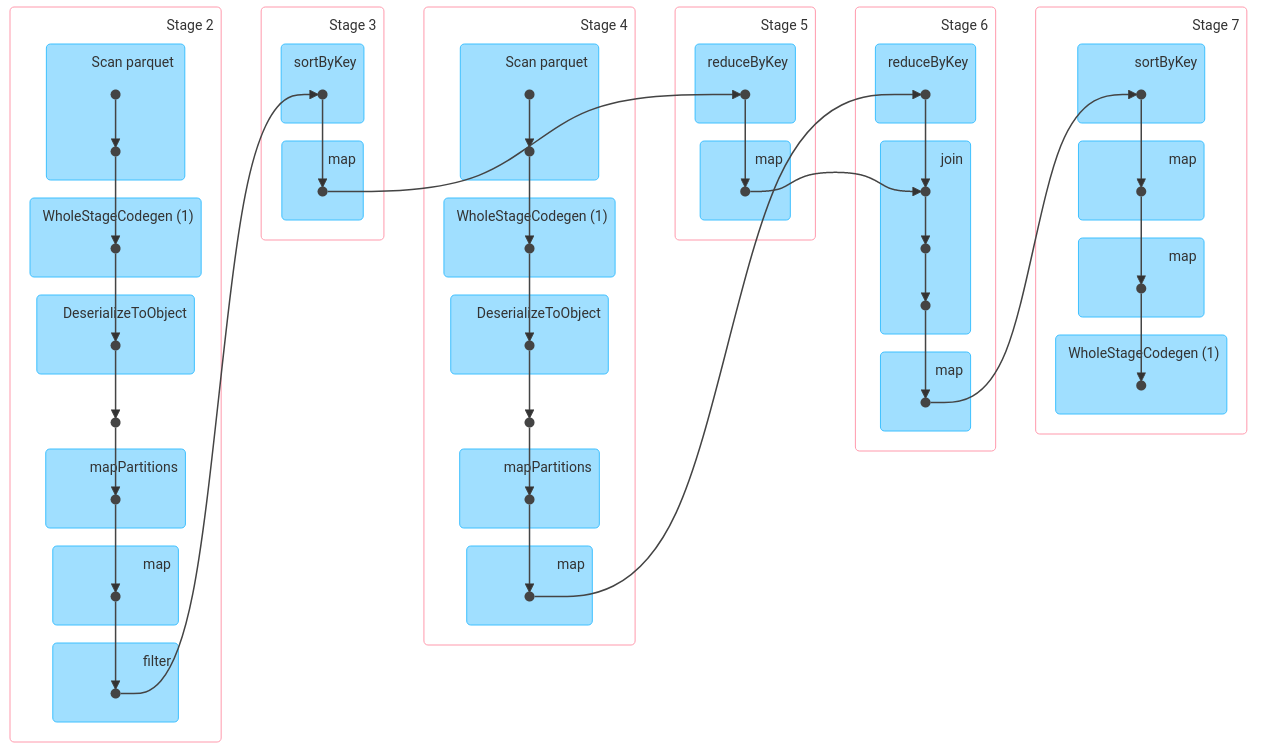
\includegraphics[scale=0.20]{Screenshot/Query1_DAG.png}
\caption{DAG query 1}\label{Query1_DAG}
\label{fig}
\end{figure}
\begin{figure}[htbp]
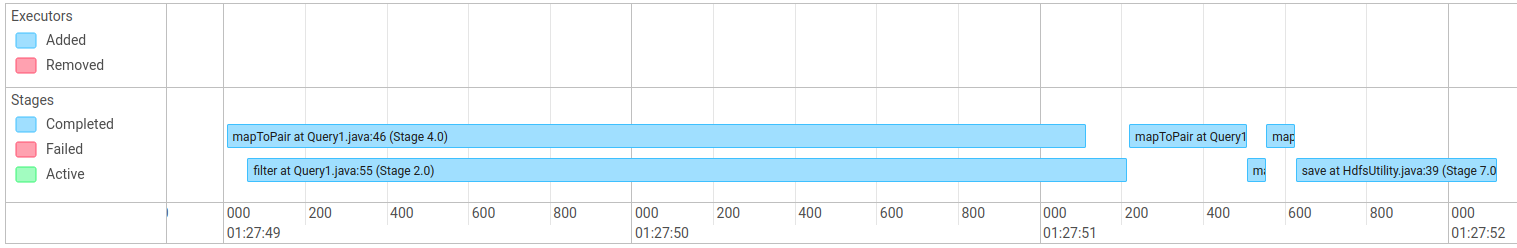
\includegraphics[scale=0.165]{Screenshot/Query1_timeline.png}
\caption{Event Timeline query 1}\label{Query1_TL}
\label{fig}
\end{figure}

\subsection*{\textbf{Query 2}}
Relativamente alla seconda \emph{query} \`{e} stato utilizzato il file \textit{somministrazioni-vaccini-latest.parquet}, il quale, in seguito al caricamento da \emph{HDFS}, \`{e} stato trasformato in \texttt{JavaPairRDD}. Durante questa fase sono state scartate le colonne irrilevanti ai fini della richiesta. La \emph{trasformazione "filter"} ha permesso l'eliminazione delle entry relative a date precedenti al 1 Febbraio 2021 e successivi al 1 Giugno 2021. Considerando come chiave la tupla \emph{area, data e fascia anagrafica} sono stati sommati i vaccini relativi ad aziende farmaceutiche differenti, ordinando, in seguito, per data. La \emph{trasformazione "groupByKey"} \`{e} stata applicata al fine di raggruppare tutte le tuple \emph{data, numero somministrazioni giornaliere} relative ad una certa regione e fascia anagrafica. Per ogni mese \`{e} stato eseguito una operazione di inserimento di date e valori macanti ed \`{e} stata effettuata \emph{regressione lineare}, in modo da prevedere il numero di donne vaccinate al primo giorno del mese successivo. Quest'ultimo passo ha previsto operazioni di raggruppamento e ordinamento. Il modello di regressione lineare \`{e} stato addestrato attraverso l'implementazione fornita dalla libreria di regressione di \texttt{Apache Commons}.
\par In figura~\ref{Query2_DAG} e~\ref{Query2_TL} \`{e} possibile osservare rispettivamente il \emph{DAG} e \emph{l'event timeline} relativi alla seconda \emph{query}. 
\begin{figure}[htbp]
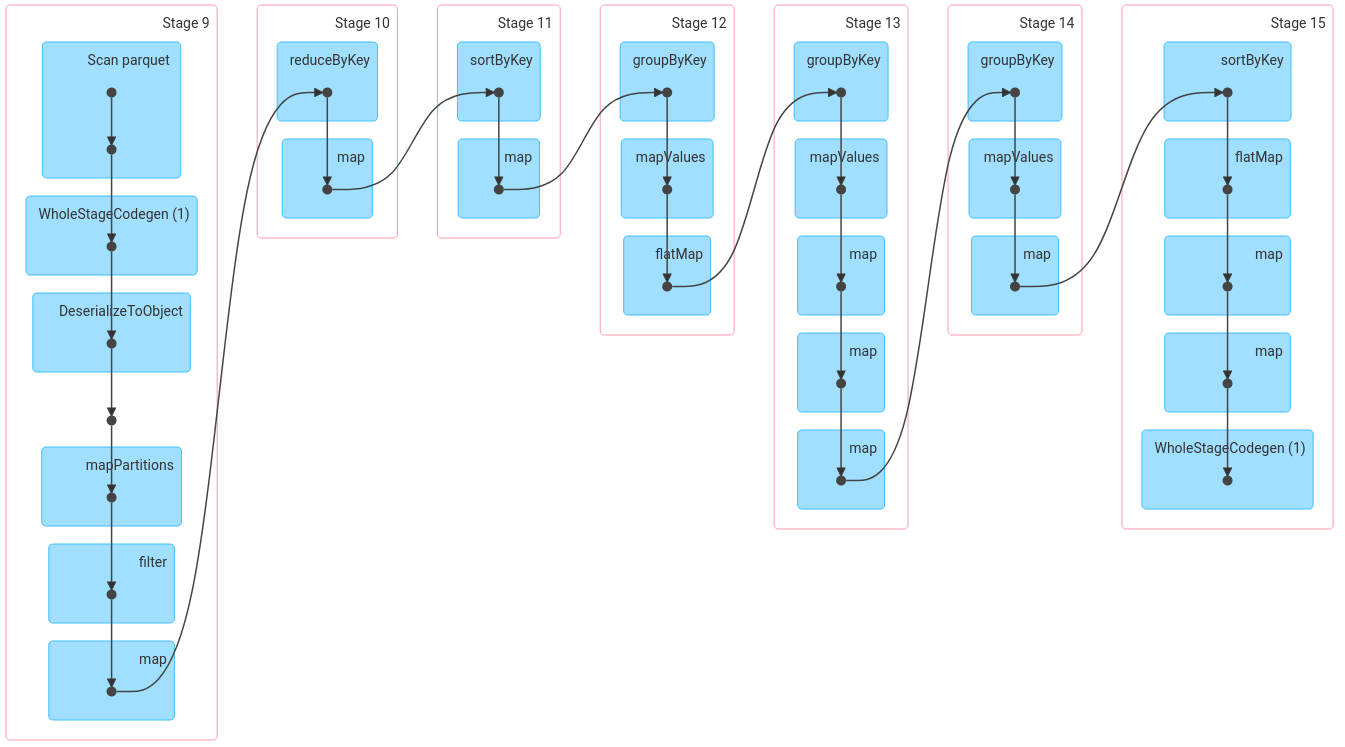
\includegraphics[scale=0.19]{Screenshot/Query2_DAG.png}
\caption{DAG query 2}\label{Query2_DAG}
\label{fig}
\end{figure}
\begin{figure}[htbp]
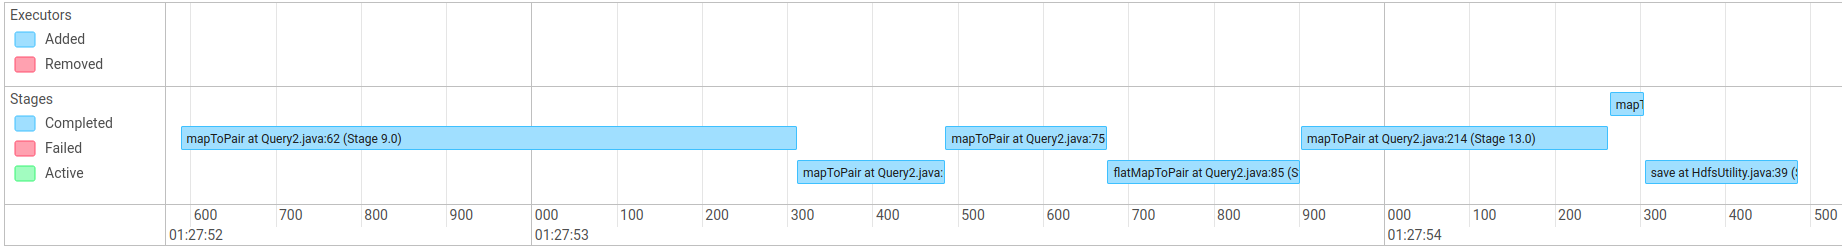
\includegraphics[scale=0.135]{Screenshot/Query2_timeline.png}
\caption{Event Timeline query 2}\label{Query2_TL}
\label{fig}
\end{figure}

\subsection*{\textbf{Query 3}}
L'ultima \emph{query} fa uso dei dati presenti nei file \textit{somministrazioni-vaccini-summary-latest.parquet} e \textit{totale-popolazione.parquet}. In seguito \`{e} stato effettuato il caricamento dei file e la trasformazione in \texttt{JavaPairRDD}. Sui dati relativi a \textit{somministrazioni-vaccini-summary-latest} si \`{e} proceduto al raggruppamento delle tuple \emph{data, numero somministrazioni giornaliere} per ogni regione, questa operazione ha permesso di svolgere regressione lineare su tutti i giorni dal 27 Dicembre 2020 al 31 Maggio 2021, in modo da prevedere il numero di vaccini effettuati in data 1 Giugno 2021. Una \emph{"reduceByKey"}, sulle regioni del medesimo file, ha, invece, permesso di calcolare il totale di vaccini effettuati dal 27 Dicembre 2020 al 31 Maggio 2021. Infine, l'operazione di somma tra le proiezioni e il totale calcolato, consentita dall'operazione di \emph{"join"}, ha decretato il numero totale previsto di vaccinati per regione al 1 Giugno 2021. Il \emph{"join"} tra l'\emph{RDD} in questione e quello contenente il numero totale di abitanti residenti in ciacuna regione (\textit{totale-popolazione}), he reso possibile calcolare la percentuale prevista di vaccinati complessivi al 1 Giugno 2021. Utilizzando due modelli presenti in \emph{MLLib}, \`{e} stato effettuato \emph{clustering} utilizzando i risultati precedenti come dataset, con numero di cluster variabile da 2 a 5. Gli algoritmi utilizzati sono \emph{K-means} e \emph{Bisecting K-means}, mentre per la regressione \`{e} stata utilizzata l'implementazione fornita dalla libreria di regressione di \texttt{Apache Commons}.
\par In figura~\ref{Query3_DAG} e~\ref{Query3_TL} \`{e} possibile osservare il \emph{DAG} e \emph{l'event timeline} relativi alla terza \emph{query}. In riferimento agli stage 18 e 19 del DAG, \`{e} possibile notare l'uso dell'operazione \texttt{cache} sull'\emph{RDD} filtrato relativo a \textit{somministrazioni-vaccini-summary-latest}, per via dell'impiego indipendente di quest'ultimo negli stage 20 e 21. Come si pu\`{o} inferire dall'\emph{event timeline}, alcuni stage vengono eseguiti parallelamente.  
\begin{figure}[htbp]
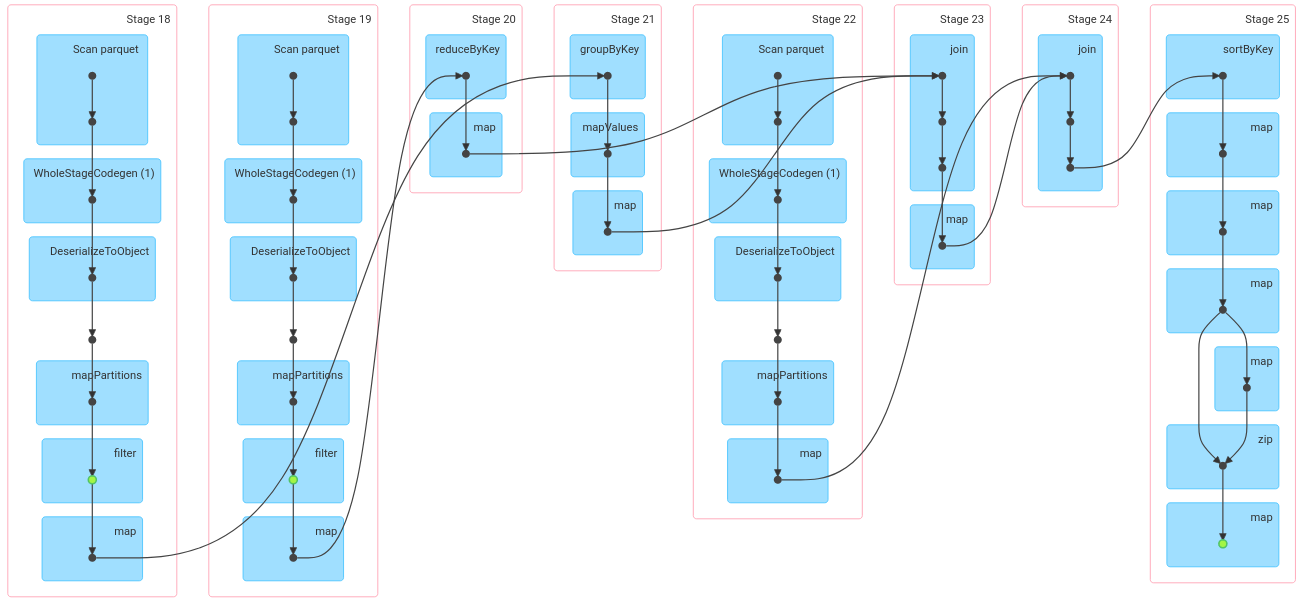
\includegraphics[scale=0.196]{Screenshot/Query3_DAG.png}
\caption{DAG query 3}\label{Query3_DAG}
\label{fig}
\end{figure}
\begin{figure}[htbp]
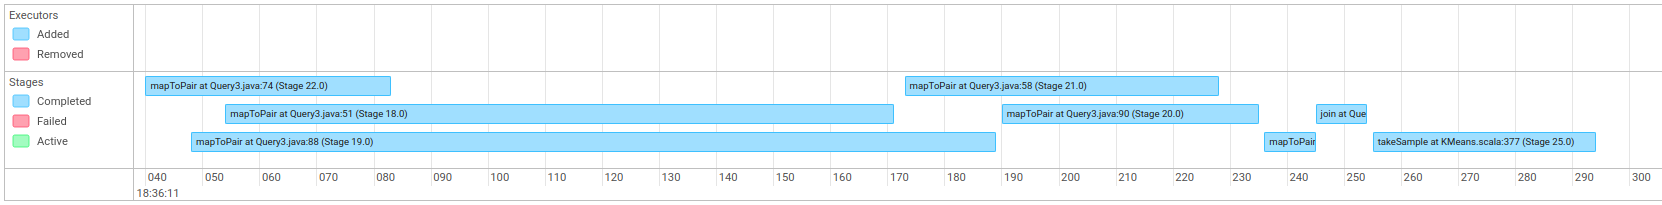
\includegraphics[scale=0.15]{Screenshot/Query3_timeline.png}
\caption{Event Timeline query 3}\label{Query3_TL}
\label{fig}
\end{figure}

\section{\textbf{Benchmark}}
L'esecuzione del progetto e la valutazione delle prestazioni sono state eseguite su \emph{Linux Xubuntu} basato su \emph{Ubuntu 20.04 LTS} virtualizzato tramite \emph{VBox}, \emph{CPU AMD Ryzen 5 3600}, 6 core, 12 thread (di cui 10 assegnati alla VM) e 16 GB di RAM (di cui 9 assegnati alla VM), con archiviazione su \emph{SSD}. \\
\begin{table}[htbp]
\caption{Tempi esecuzione query}
\begin{center}
    \begin{tabular}{|c|c|c|}
    \hline
    \textbf{Query} & \textbf{Media} & \textbf{Varianza}  \\ \hline
    Query 1 & 221.1 & 41.1  \\ \hline
    Query 2 & 925.2 & 34.2 \\ \hline
    Query 3 & 2778.4 & 260.3 \\ \hline
    \multicolumn{3}{l}{$^{\mathrm{*}}$I tempi sono espressi in millisecondi.}
    \end{tabular}
\label{tab1}
\end{center}
\end{table}
\par In tabella~\ref{tab1} sono riportati i tempi di processamento delle query. Sono state considerate le performance al netto di startup della \emph{Java Virtual Machine} su cui \emph{Spark} opera e caricamento dei file dall'\emph{HDFS}. I tempi scrittura dei risultati sul \emph{file system distribuito}, invece, sono stati considerati, in modo da rendere effettive tutte le operazioni (trasformazioni) eseguite da \emph{Spark}. Come si pu\`{o} notare, la query 3 risulta molto pi\`{u} lenta delle altre due, che, invece, mostrano risultati migliori. Tale evidenza \`{e} causata dall'inclusione, nel totale, dei tempi di addestramento degli algoritmi di \emph{clustering}, che possono essere osservati in tabella~\ref{tab2}.
\begin{table}[htbp]
\caption{Tempi esecuzione clustering}
\begin{center}
\begin{tabular}{|c|c|c|c|c|}
\hline
\textbf{}&\multicolumn{4}{|c|}{\textbf{Modello}} \\ \hline
\textbf{Numero} & \multicolumn{2}{|c|}{\textbf{K-means}} & \multicolumn{2}{|c|}{\textbf{Bisecting K-means}} \\ \cline{2-5} 
\textbf{cluster} & \textbf{Media} & \textbf{Varianza} & \textbf{Media} & \textbf{Varianza} \\ \hline
2 & 347.3 & 43.6 & 203.2 & 62.4 \\ \hline
3 & 136.2 & 21.6 & 127.1 & 24.8 \\ \hline
4 & 153.1 & 39.5 & 148.2 & 25.5 \\ \hline
5 & 148.9 & 51.9 & 144.3 & 42.1 \\ \hline
\multicolumn{5}{l}{$^{\mathrm{*}}$I tempi sono espressi in millisecondi.}
\end{tabular}
\label{tab2}
\end{center}
\end{table}
\par Sempre dalla tabella~\ref{tab2} \`{e} possibile notare che i tempi di addestramento del primo modello (\emph{K-Means con numero di cluster pari a 2}) risultano superiori a quelli relativi alle successive combinazioni. Questo dovuto al caching effettuato da MLlib dopo la prima esecuzione del modello di clustering, come si evince dalla figura~\ref{Query3_skipped} che raffigura il DAG della seconda esecuzione di tale modello. 
\begin{table}[htbp]
\caption{Costo clustering: WSSSE}
\begin{center}
\begin{tabular}{|c|c|c|}
\hline
\textbf{Numero}&\multicolumn{2}{|c|}{\textbf{Modello}} \\ \cline{2-3}
\textbf{cluster} & \multicolumn{1}{|c|}{\textbf{K-means}} & \multicolumn{1}{|c|}{\textbf{Bisecting K-means}} \\ \hline
2 & 0.005392 & 0.005639 \\ \hline
3 & 0.003129 & 0.002325 \\ \hline
4 & 0.001469 & 0.001585 \\ \hline
5 & 0.000751 & 0.000751 \\ \hline
\end{tabular}
\label{tab3}
\end{center}
\end{table}
\par In tabella~\ref{tab3}, invece, \`{e} possibile osservare come il \emph{Within Set Sum of Squared Error} medio, per i due algoritmi di \emph{clustering}, decresca al crescere del numero di cluster, anche se questo non \`{e} scontato per via dell'inizializzazione randomica dei centroidi. 
\begin{figure}[htbp]
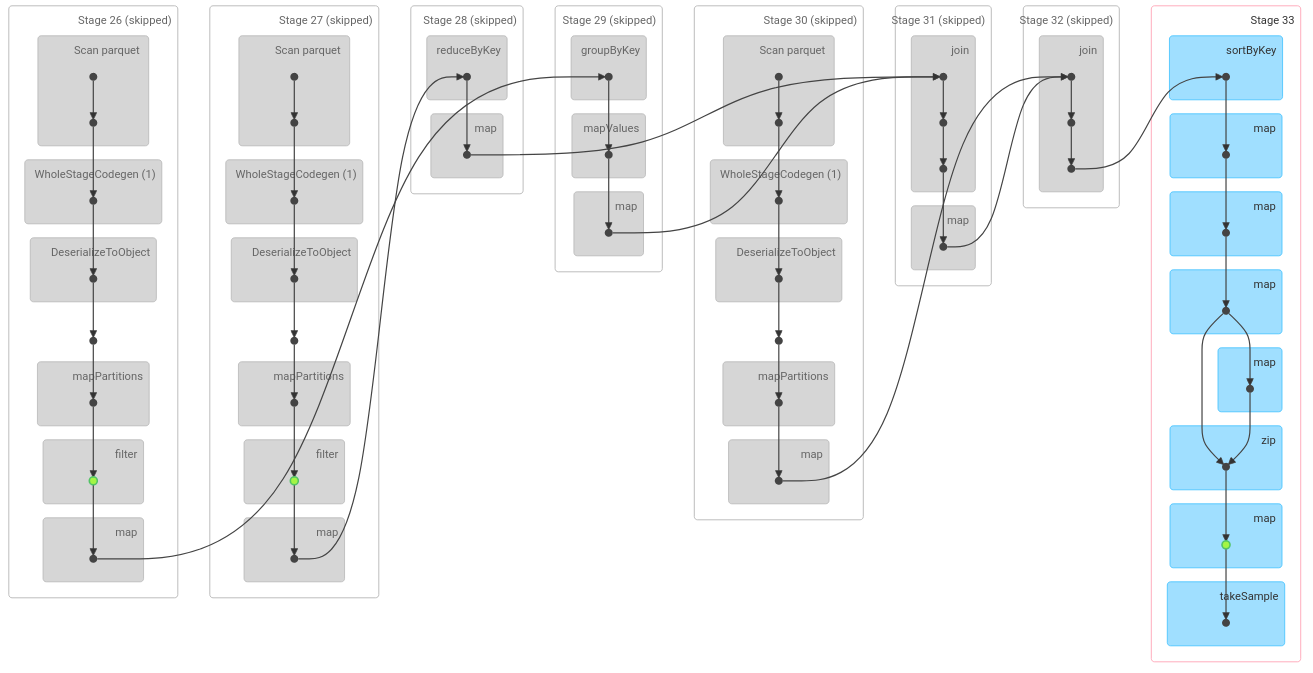
\includegraphics[scale=0.196]{Screenshot/Query3_skipped.png}
\caption{DAG query 3, secondo run cluster}\label{Query3_skipped}
\label{fig}
\end{figure}


\begin{thebibliography}{00}
\bibitem{b1} \url{https://spark.apache.org/docs/latest/}
\bibitem{b2} \url{https://stackoverflow.com/}
\bibitem{b3} \url{https://nifi.apache.org/}
\bibitem{b4} \url{https://hadoop.apache.org/docs/stable/}
\bibitem{b5} \url{http://spark.apache.org/docs/latest/ml-guide.html}
\bibitem{b6} \url{https://commons.apache.org/proper/commons-math/javadocs/api-3.3/org/apache/commons/math3/stat/regression/SimpleRegression.html}
\end{thebibliography}

\end{document}
